% !TEX encoding = UTF-8 Unicode

% Beispiel für ein LaTeX-Dokument im Format "seminarvorlage"
\documentclass[ngerman]{seminarvorlage}
% ngerman = Deutsch in neuer Rechtschreibung, alternativ english
\usepackage[utf8]{inputenc} % Kodierung der Umlaute
\usepackage{babel} % automatische Sprachanpassung, Sprache siehe oben
\usepackage{cleveref} % für bequeme Referenzen, siehe \cref unten

%Own Code
\newcommand*{\fullref}[1]{\hyperref[{#1}]{\autoref*{#1} \nameref*{#1}}} % One single link
\newcommand*{\quelle}{% 
  \footnotesize Quelle: 
} 

\begin{document}

% Unbedingt angeben: Titel, Autoren, E-Mail
% Freiwillig: Adresse
\title{Embedded Realtime OS FreeRTOS auf STM32F4}
\numberofauthors{2}
\author{
  \alignauthor Michael Ebert\\
		\affaddr{Ad-hoc Networks GmbH}\\
    \email{ebert@ad-hoc.network}
  \alignauthor Christoph Bläßer\\
		\affaddr{Bundesamt für Sicherheit in der Informationstechnik}
    \email{christoph.blaesser@gmx.de}
}

\maketitle
\keywords{RTOS, FreeRtos, ARM , STM32, Real Time.}

\abstract{
Im Rahmen des vorliegenden Papers wird das Echtzeitbetriebssystem FreeRtos vorgestellt. Hierzu werden zu Beginn die allgemeinen Vorgaben für Echtzeitbetriebssysteme beschrieben. Im Verlauf des Textes wird an ausgewählten Beispielen dargestellt, wie FreeRos diese Anforderungen berücksichtigt und durch geeignete Programmfunktionen umsetzt.

}
\section{Grundlagen}
\subsection{Allgemeine Anforderungen an Betriebssysteme}
Betriebssysteme verwalten den Hardwarezugriff und stellen sicher, dass eingesetzte Software die benötigte Rechenzeit zur Verfügung gestellt bekommt. Gleichzeitig regeln Sie den Hardwarezugriff und organiseren den konkurierenden Zugriff, beispielsweise auf Netzwerkkarten und Festplatten. Sie stellen Funktionen für die Interprozesskommunikation bereit udn übernehmen grundlegende Aufgaben wie die Organisation von Arbeitsspeicher.

%%Brauchen wir das ? trifft auf ein RTOs im prinzip nicht zu, konkurierender Zugriff auf externe Ressourcen muss bei einem RTOS durch den Entwickler sichergestellt werden. Die einzigen Resourcen die ein RTOS verwaltet ist Zeit + Heap(teilweise) 
\subsection{Echtzeitsysteme und Echzeitbetriebsysteme}
Mit der steigenden Leistungsfähigkeit von modernen $\mu$ Prozessoren, steigen auch die Anforderungen an die Software die auf diese Systeme aufsetzt. Viele dieser Systeme verlangen trotz ihrer Komplexität, dass Teile des Programmablauf in bestimmten zeitlichen Grenzen ausgeführt wird und somit vorhersehbar und deterministisch sind. Systeme die eine solche Anforderung unterliegen werden Echtzeitsysteme genannt. Echtzeitsysteme unterliegen einer weiteren Unterteilung in weiche Echtzeitsystem (soft realtime systems) und harte Echtzeitsysteme (hard realtime systems). Ein weiches Echtzeitsysteme soll eine Aufgabe in den vorgegeben zeitlichen Grenzen ausführen, ein über\-schreiten ist aber erlaubt und führt nicht unmittelbar zu einem Fehler. Ein hartes Echtzeitsystem hingegen muss die gestellte Aufgabe in den vorgegebenen Grenzen ausführen. Eine Überschreitung macht das System unbrauchbar. Einige Beispielsysteme und deren Echtzeitzuordnung wir in Tabelle \ref{tab:BeispieleEchzeitsystem} gezeigt. Um die grundsätzliche Funktionalität eines Echtzeitbetriebssystems zu erläutern, müssen zu erst die Grundmodelle für den Programmablauf eingebetter Systeme beschrieben werden. Der Programmablauf eingebetteter Systeme lässt sich auf drei Modelle zurückführen (Abbildung \ref{fig:Programmablauf}). Eingebettete Anwendungen können in einer einzigen Schleife (mit oder ohne Interrupt Unterbrechungen) laufen oder aber in event-gesteuerten nebenläufigen eigenständigen Programmabschnitten (Thread oder Task\footnote{Nachfolgenden wird Task benutzt, da dies der geläufige Begriff bei FreeRtos ist. In der Literatur zu Echtzeitsystemen ist der Begriff nicht exakt definiert.}) ausgeführt werden. Die nebenläufige Ausführung der unterschiedlichen Programmsegmente ist nur durch einen RTOS-Kernel (Scheduler) zu erreichen. Ein RTOS Kernel abstrahiert Timing Informationen und kümmert sich darum, dass die nächste Task rechtzeitig ausgeführt wird. Der Entwickler ist dafür verantwortlich, dass die Task die gewünschte Aufgabe im zeitlichen Rahmen ausführt. Wie sichergestellt werden kann, dass eine Task  harten oder weichen Echtzeitanforderungen entspricht wird Abschnitt \ref{sec:Echtzeitanalyse} beschrieben. Für viele kleine Anwendungen kann die Nutzung einer einzigen Schleife durchaus sinnvoll sein, sollten beispielsweise die Ressourcen so knapp sein, dass ein Overhead an Funktionalität ausgeschlossen werden muss. Ein großer Nachteil der "`einschleifen Variante"' ist die permanente Nutzung des Prozessors. Besonders bei akkubetriebenen Geräten wie IoT Devices oder Mobiltelefonen wird sehr genau auf die Energieaufnahme geachtet. Ein RTOS bietet hingegen Funktionen mit denen sehr leicht ermittelt werden kann, ob ein Gerät in einen Schlafmodus wechseln kann, dies wird in Abschnitt \ref{sec:Low Power Modes} an Beispielen von FreeRtos und einem ARM $\mu$Prozessor demonstriert. Neben der Echtzeitfähig gibt es aber noch viele weitere Vorzüge für den Einsatz eines Echtzeitbetriebssystems.  
Durch das Herunterbrechen der Anwendung in Task entstehen viele kleine Module, die jeweils eine kleine Teilaufgabe des Gesamtsystems übernehmen.Durch ein sauber definiertes Interface zur Kommunikation der Tasks, lässt sich die Entwicklungsarbeit leicht auf mehrere Entwickler-Teams verteilen. Dies ermöglicht auch den Einsatz von agilen Entwicklungsmethoden wie Scrum in der Entwicklung von eingebetteten Systemen.  
\newline
TODO Überleitung FreeRtos
\newline  
\begin{figure}
	\centering
		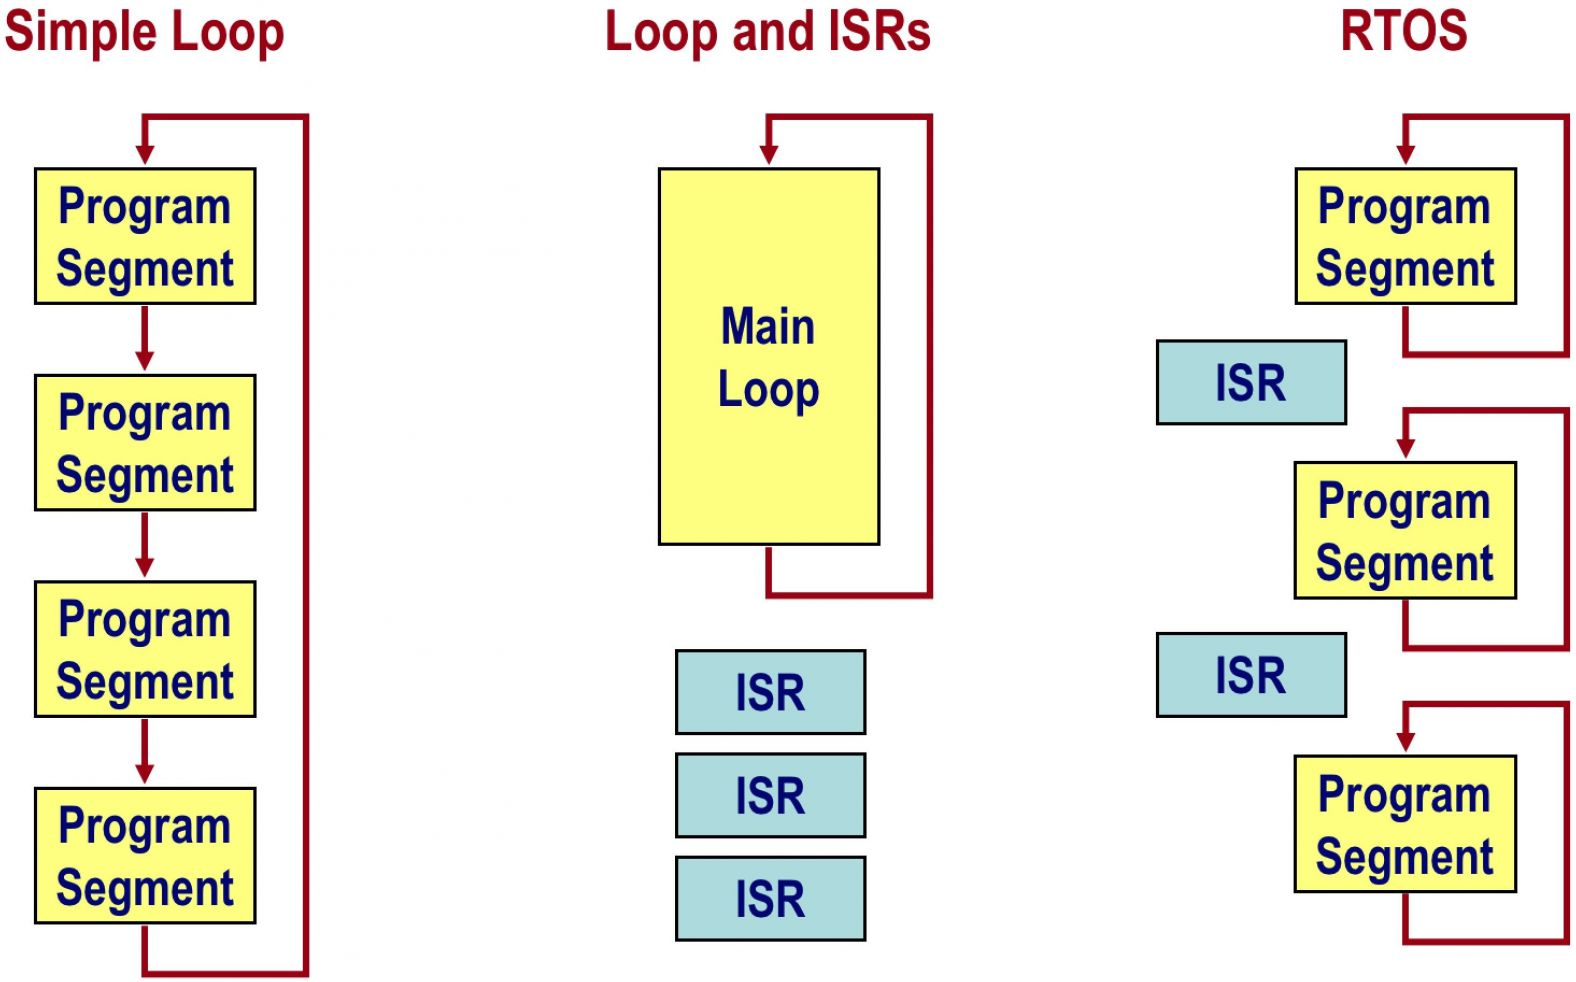
\includegraphics[width=0.3\textwidth]{Pictures/EmbeddedCom/cwrtos2f5c.jpg}
	\caption{Übersicht Programmabläufe}
	\quelle\url{http://www.embedded.com/}
	\label{fig:Programmablauf}
\end{figure}

\begin{table*}
	\centering
		\begin{tabular}{|l|l|}
		\hline
			   Beispiel & Echtzeit Typ \\
				\hline
  Tastatur Controller & Soft Realtime \\
	\hline
  Echtzeit Media Streaming  & Soft Realtime \\
	\hline
	Controller CD Laufwerk  & Hard Realtime \\
	\hline
	Airbag System  & Hard Realtime\\
	\hline
		\end{tabular}
	\caption{Beispiele Echzeitsystem}
	\label{tab:BeispieleEchzeitsystem}
\end{table*}



\subsection{Einsatzgebiet und Beispielanwendung}
%Echtzeitbetriebssysteme kommen zum Einsatz wenn neben den oben genannten Anforderungen an ein normales Betriebssystem weitere Anforderungen gestellt werden, die ein normales Betriebssystem nicht berücksichtigt. Dies können beispielsweise garantiert berechenbare Reaktionszeiten sein wie sie in der Fabrikation oder im Automobilbereich gefordert werden oder geringe Leistungsaufnahmen wie bei Komponenten des Internet of Things (IoT). Insgesamt wird zwischen Harten und Weichen Echtzeitkriterien unterschieden. Diese Gliedern sich wie folgt:\newline
%%%Zitat Anfang
%\begin{itemize}
	%\item Antwortzeiten
	%\item Start-zu-Start Jitter von Tasks und Software-Komponenten
	%\item Mehrfachaktivierung von Tasks
	%\item Ausführungsreihenfolge von Software-Komponenten
	%\item Latenzen von Wirkketten (Event Chains)
	%\item Verlust von Daten
	%\item Alter der Daten
	%\item Datenkonsistenz
	%\item Wiederverwendung von Daten
	%\item Verlust von Interrupts
	%\item Blockierung von Interrupts
%\end{itemize}
%%%Zitat Ende Quelle: http://www.inchron.com/fileadmin/INCHRON/3-PDFs/EN/Paper_IAV_Tagung_Sim_u_Test_B_Mai10_pdf.pdf
%
%
%Aufgrund der Eingangs geschilderten Einsatzbereiche ist leich zu erkennen, dass Echzeitbetriebssysteme häufigin Umgebungen zum Einsatz kommen, in denen besondere Anforderungen an die Hardware gestellt werden. Häufig verfügt die Hardware nur über begrenzte Speicherkapazitäten, über geringe Wärmeableitfähigkeiten und damit geringe Rechenleistung. Die zur Verfügung stehende Energie muss bei der Entwicklung ebenfalls berücksichtigt werden. 
%Vor diesem Hintergrund benötigen Echtzeitbetriebssysteme nur wenig Speicherplatz und implementieren Funktionen um den Prozessor und die angeschlossene Peripherie nur kurzzeitig zu belasten und in der restlichen Zeit in den Ruhezustand zu verseten.

\section{FreeRtos} 
\subsection{Geschichte}
\subsection{Zielsysteme STM32F4 (ARM Cortex M3)}
\subsection{Entwicklungsumgebung}
FreeRtos ist im Prinzip nicht an eine spezielle Entwicklungs\-umgebung gebunden. Bevor eine Ent\-wicklung beginnt ist es dennoch rat\-sam sich einen Über\-blick über die verfügbaren IDEs zu machen. Der wichtigste Punkt der hier zu nennen ist, ist das Debugging. Da ein Echtzeitbetriebssystem eine weitere Abstraktionsebene hinzufügt und wie eine Art Middleware fungiert, lassen Sich viele RTOS spezifische Funktionen und Eigenschaften wie Queues, Task Stacks etc. nur mühsam mit einem Debugger wie GDB oder OpenOCD untersuchen. Viele der marktgängigen Entwicklungsumgebungen bieten daher spezielle RTOS aware Pakete, so dass ein einfacherer Zugriff auf RTOS Objekte und Eigenschaften möglich ist. Wie die RTOS awareness beim Debugging eingesetzt wird und welche Funktionalitäten sie einem Entwickler bietet wird in Abschnitt \ref{sec:Debugging von Echtzeitsystemen} aufgezeigt. Ein weiterer Punkt der bei der Auswahl der IDE getroffen werden muss sind die Kosten. Bei Propritäre IDEs können oft mehrere tausend Euro Lizenzkosten anfallen, bieten aber den Vorteil der nahtlosen Einbindungen von $\mu$Prozessoren und Echtzeitbetriebssystem (RTOS awareness). Bei der Entwicklung von ARM uProzessoren sind hier Keil (Arm), IAR Workbench und True Studio (Atollic) zu nennen. Diese Entwicklungsumgebungen lassen sich zum Teil auch frei verwenden, allerdings mit starken Einschränkungen wie z.B. maximal Codesize. Auf der nicht proprietären Seiten steht Eclipse CDT zur Verfügung, es ist komplett frei in der Verwendung und hat keine Beschränkungen. Nachteil ist hier das die Integration nicht so einfach ist wie bei den anderen IDEs. RTOS awarness wird bei Eclipse durch die Installation weiterer Plugins erreicht. Ein weiterer Nachteil ist, dass es keine Beispielprojekte für Eclipse CDT und FreeRtos zur Verfügung stehen, daher müssen Projekte von Grund auf selbst konfiguriert und installiert werden. Da im Laufe dieser Arbeit Eclipse CDT für alle Beispiele verwendet wird, wird in Abschnitt \ref{sec:Einrichtung und Konfiguration} das Aufsetzen einer Basiskonfiguration erklärt.       
\subsection{Einrichten und Konfiguration}
\label{sec:Einrichtung und Konfiguration}
%%Ordner und Dateistruktur
\subsection{Memory Allocation}
Beim erzeugen von Rtos Objekten wie Tasks, Queues oder Semaphore wird Speicher im RAM benötigt. Für dynamische Speicherzuweisung wird in einfachen Embedded Anwendungen die Standard C Funktion malloc() und free() verwendet. Für Echtzeitsysteme die auf einem RTOS aufsetzen sind diese Funktionen aber nicht zu empfehlen. Folgende Eigenschaften\cite{MasteringFreeRtos} machen Sie unbrauchbar:
\begin{itemize}
	\item nicht thread safe
	\item nicht deterministisch
	\item tendieren zur Fragmentierung des RAM
	\item schwer zu debuggen
	\item Bibliotheksfunktionen benötigen viel Speicher
\end{itemize}
Des Weiteren verlangen viele embedded Anwendungen Zertifikate (z.B. Militärische Anwendungen) die ein dynamische Speicherverwaltung durch malloc() und free() verbieten, oder aber sogar nur statische Speicherverwaltung zur Compilezeit zulassen. In FreeRtos werden die Echtzeitanforderungen an die Speicherverwaltung dadurch erreicht, dass malloc() und free() durch die Funktionen pvPortMalloc() und pvPortFree() ersetzt werden. Die Funktionsdefinition kann vielfältig sein, zum Einen bietet FreeRtos fünf Basis Heap (Heap1.c bis Heap5.c) Implementierungen und zum Anderen ist es auch möglich diese Funktionen selbst auszuimplementieren. TODO    

\subsubsection{Memory Protection}
\subsection{Scheduling}

\subsection{Intertask Kommunikation}
\subsection{Interrupt Handling}
\subsection{Low Power Modes auf Stm32F4}
\label{sec:Low Power Modes} 
\section{Komplexität durch Nebenläufigkeit}
\section{Debugging von Echtzeitsystemen} 
\label{sec:Debugging von Echtzeitsystemen}
\section{Echtzeitanalyse}
\label{sec:Echtzeitanalyse} 

 
\section{Zusammenfassung}
\pagebreak
\bibliographystyle{abbrv}
\bibliography{literatur} % Daten aus der Datei literatur.bib verwenden.
\end{document}

